% asset_id: FA22LinearCombinationsOfIndependentVariablesTikZ-002
% unit_code: FA22
% topic_code: FA22-LINCOMB
% topic_id: FA22LinearCombinationsOfIndependentVariables
% source: Phase 1 visual placeholder register
% purpose: Scaling random variables
\documentclass[tikz,border=10pt]{standalone}
\usepackage{amsmath}
\usepackage{tikz}
\begin{document}
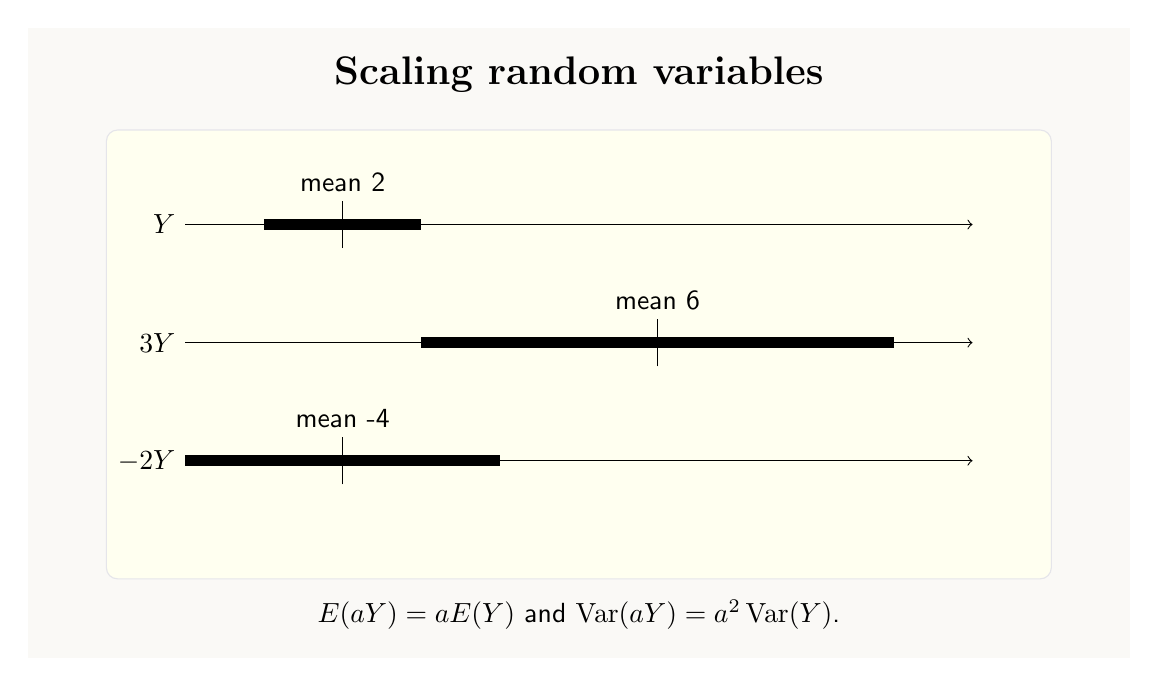
\begin{tikzpicture}[font=\sffamily]
\fill[fill={rgb,255:red,250;green,249;blue,246}] (-1,-1) rectangle (13,7);
\node[font=\bfseries\Large] at (6,6.4) {Scaling random variables};
\draw[rounded corners, fill={rgb,255:red,255;green,255;blue,240}, draw={rgb,255:red,229;green,229;blue,234}] (0,0) rectangle (12,5.7);

\draw[->] (1,4.5)--(11,4.5); \node[left] at (1,4.5) {$Y$};
\draw[line width=4pt] (2,4.5)--(4,4.5); \draw (3,4.2)--(3,4.8); \node[above] at (3,4.8) {mean 2};
\draw[->] (1,3)--(11,3); \node[left] at (1,3) {$3Y$};
\draw[line width=4pt] (4,3)--(10,3); \draw (7,2.7)--(7,3.3); \node[above] at (7,3.3) {mean 6};
\draw[->] (1,1.5)--(11,1.5); \node[left] at (1,1.5) {$-2Y$};
\draw[line width=4pt] (1,1.5)--(5,1.5); \draw (3,1.2)--(3,1.8); \node[above] at (3,1.8) {mean -4};
\node at (6,-0.45) {$E(aY)=aE(Y)$ and $\operatorname{Var}(aY)=a^2\operatorname{Var}(Y)$.};

\end{tikzpicture}
\end{document}
